\section{Scope}
\label{sec:scope}

The \textit{\textbf{scope}} of a declaration is the portion of the program text over which the declaration is effective. Similarly, the \textit{\textbf{scope}} of a binding is the portion of the program text over which the binding applies.

In some early programming languages, the scope of each declaration was the whole program. In modern languages, the scope of each declaration is influenced by the program’s syntactic structure, in particular the arrangement of blocks.

\subsection{Block Structure}

A \textit{\textbf{block}} defines the scope of the identifiers declared
inside (boundary of the definition validity). For variables, they
also define the lifetime. Each programming language has its own forms of blocks:
\begin{itemize}
  \item The blocks of a \texttt{C} program are block commands (\{ ... \}), function bodies, compilation units (source files), and the program as a whole.
  \item The blocks of a \texttt{JAVA} program are block commands ({ ... }), method bodies, class declarations, packages, and the program as a whole.
  \item The block of a \texttt{Haskell} program are `\texttt{let \textit{definitions} in \textit{expression}}' defines a block expression. Also `\textit{expression} \texttt{where} \textit{definitions}' defines a block expression. (the definitions have a local scope and not accessible outside of the expression).
\end{itemize}

Block structure of the language is defined by the organization of the blocks.

\newpage

\subsubsection{Monolithic Block Structure}

In a language with \textit{\textbf{monolithic block structure}}, the only block is the whole program, so the scope of every declaration is the whole program. In other words, all declarations are global.
\begin{figure}[H]
  \centering
  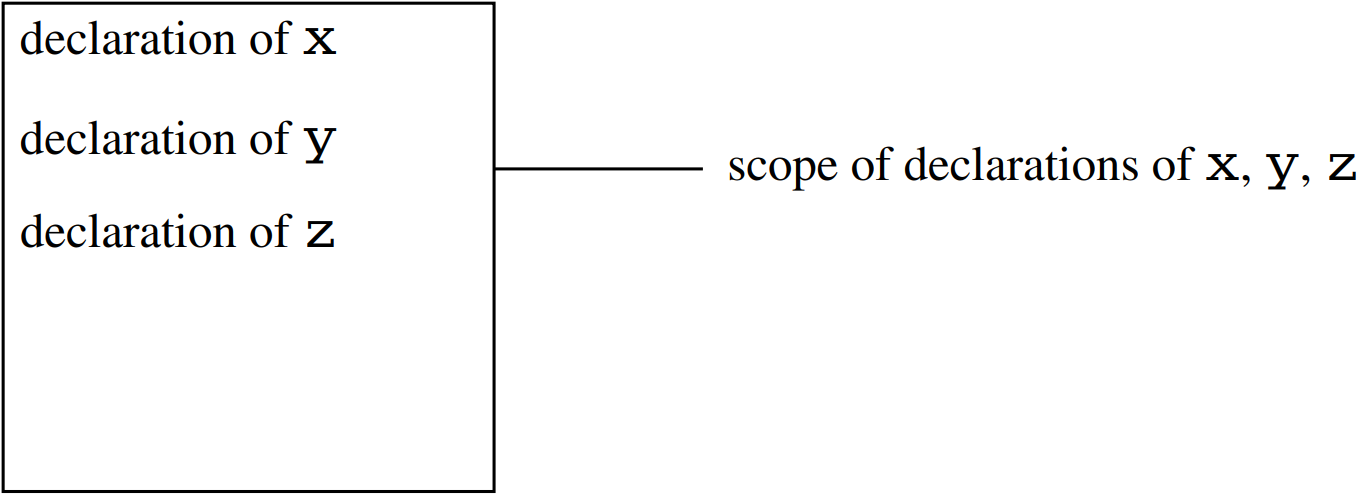
\includegraphics[width=\linewidth]{img/fig-4.1.png}
  \caption{Monolithic block structure.}
  \label{fig:fig1}
\end{figure}
In a long program with many identifiers, they share the same scope and they need to be distinct.

\subsubsection{Flat Block Structure}

In a language with \textit{\textbf{flat block structure}}, the program is partitioned into several non-overlapping blocks. In other words, program contains \textit{the global scope and only a single level local scope of function definitions}. No further nesting is possible.

\begin{figure}[H]
  \centering
  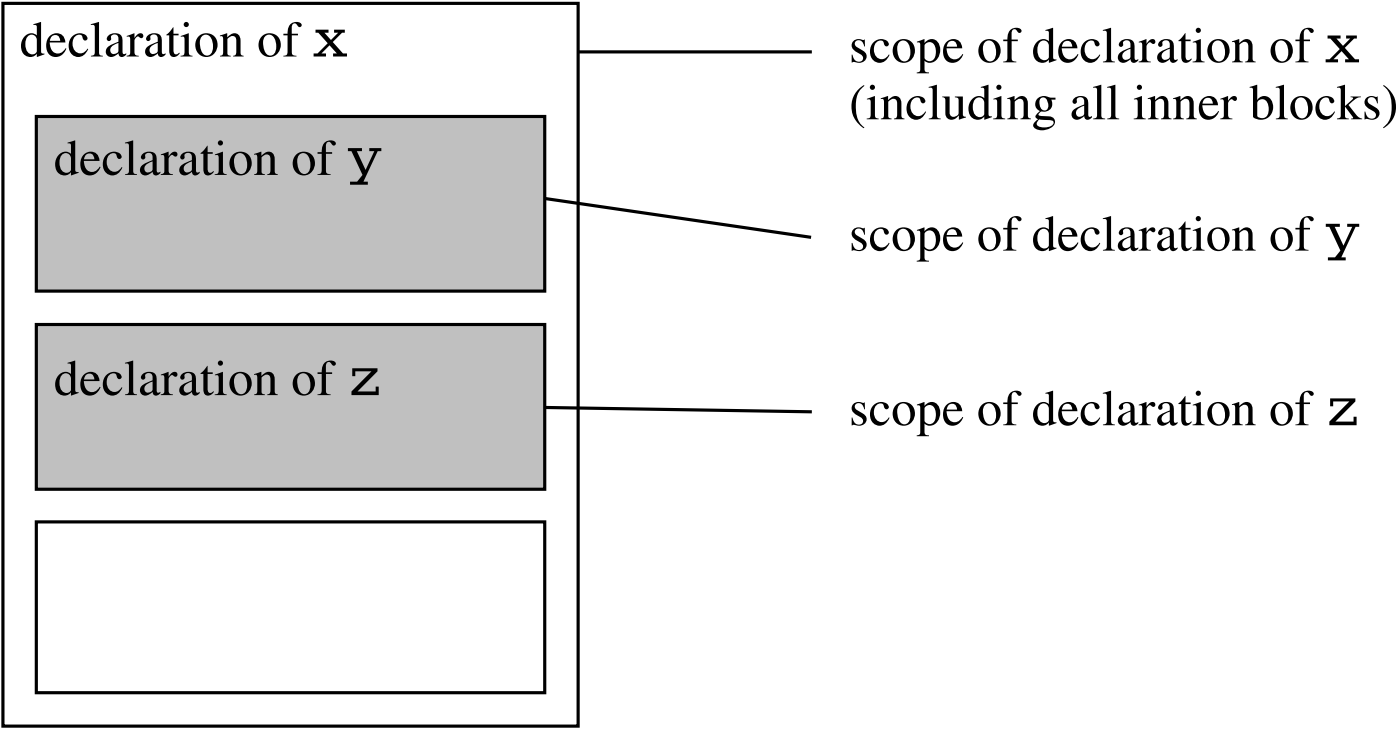
\includegraphics[width=\linewidth]{img/fig-4.2.png}
  \caption{Flat block structure.}
  \label{fig:fig2}
\end{figure}

\subsubsection{Nested Block Structure}

In a language with \textit{\textbf{nested block structure}}, blocks may be nested within other blocks.

\begin{figure}[H]
  \centering
  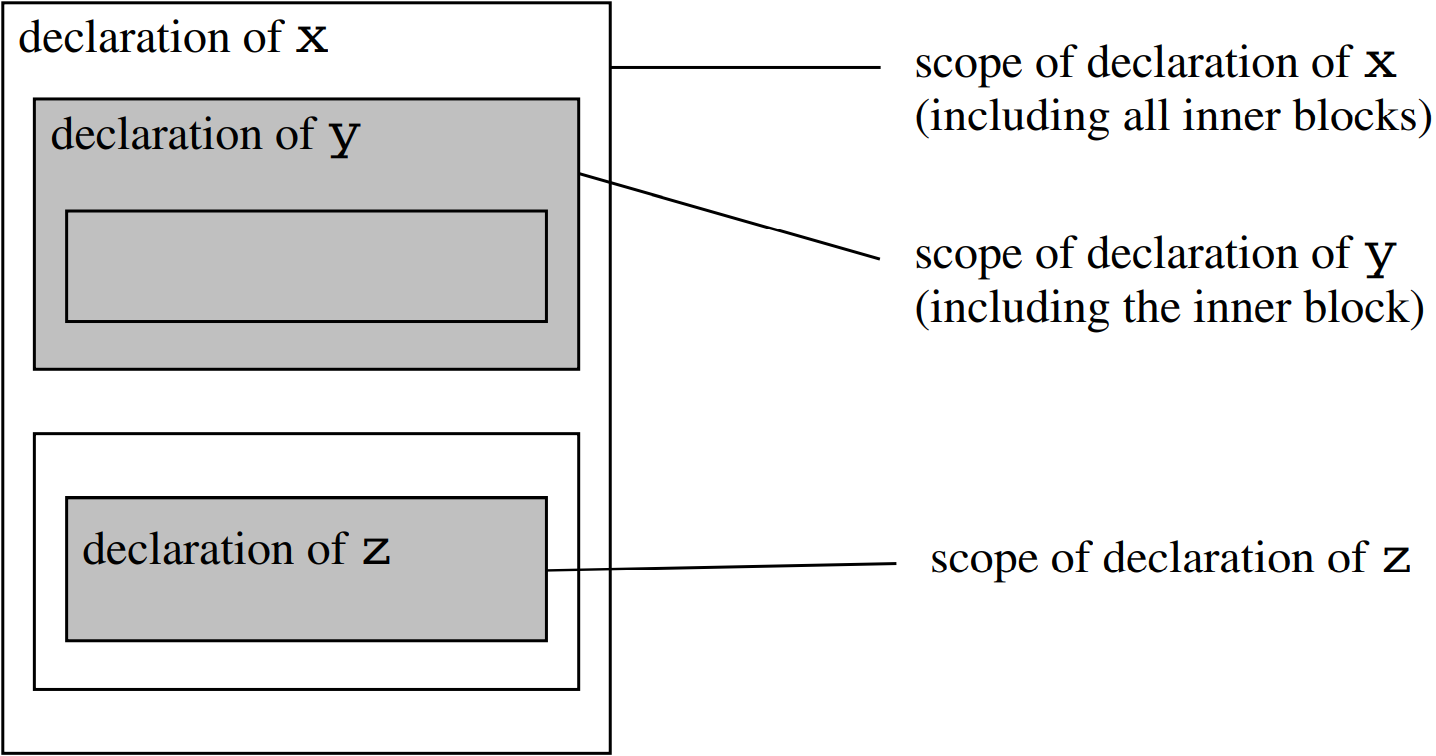
\includegraphics[width=\linewidth]{img/fig-4.3.png}
  \caption{Nested block structure.}
  \label{fig:fig3}
\end{figure}


\subsection{Scope and Visibility}

Consider all the occurrences of identifiers in a program. We must distinguish two different kinds of identifier occurrences:
\begin{itemize}
  \item A \textit{\textbf{binding occurrence}} of identifier \textit{I} is an occurrence where \textit{I} is bound to some entity \textit{X}.
  \item An \textit{\textbf{applied occurrence}} of \textit{I} is an occurrence where use is made of the entity \textit{X} to which \textit{I} has been bound. At each such applied occurrence we say that \textit{I} denotes \textit{X}.
\end{itemize}

When a program contains more than one block, it is possible for the same
identifier \textit{I} to be declared in different blocks. In general, \textit{I} will denote a different entity in each block.

Consider two nested blocks, such that the inner block lies within the scope of a declaration of identifier \textit{I} in the outer block:
\begin{itemize}
  \item If the inner block \textit{does not} contain a declaration of \textit{I}, then applied occurrences of \textit{I} both inside and outside the inner block correspond to the same declaration of \textit{I}. The declaration of \textit{I} is then said to be \textit{\textbf{visible}} throughout the outer and inner blocks.
  \item If the inner block \textit{does} contain a declaration of \textit{I}, then all applied occurrences of \textit{I} inside the inner block correspond to the inner, not the outer, declaration of \textit{I}. The outer declaration of \textit{I} is then said to be \textit{\textbf{hidden}} by the inner declaration of \textit{I}.
\end{itemize}

\begin{listing}[H]

\begin{minted}{c}
int x, y;

int f(double x) {
  ...             // parameter x hides global x
                  // in f()
}

int g(double a) {
  int y;         // local y hides global y in g()
  double f;      // local f hides global f()
                 // in g()
  ...
}

int main() {
  int y;        // local y hides global y
                // in main()
}
\end{minted}
\caption{}
\label{code:code4}
\end{listing}

\newpage

\end{multicols*}

\begin{multicols}{2}
\setlength{\columnsep}{1.5cm}
\setlength{\columnseprule}{0.2pt}

\subsection{Static vs Dynamic Scoping}

When are the binding and scope resolution done? In compile time or run
time? Two options:
\begin{enumerate}
  \item Static binding, static scope
  \item Dynamic binding, dynamic scope  
\end{enumerate}

The first defines scope and binding based on the lexical structure of the program and binding is done \textit{at compile time}. Second activates the definitions in a block during the execution of the block. The environment changes dynamically \textit{at run time} as functions are called and returned.

\vspace*{\fill}
\columnbreak

\subsubsection{Static Binding}

Programs' shape is significant. Environment is based on the position in the source (lexical scope). Most languages apply static binding (\texttt{C, Haskell, Pascal, Java, ...})

\begin{dummyenv}
\def\X{\color{green!60!black}\bf x}
\def\gX{\color{red!60!black}\bf x}
\def\Y{\color{green!60!black}\bf y}
\def\mY{\color{red!60!black}\bf y}
\def\fY{\color{yellow!60!black}\bf y}
\def\gA{\color{yellow!60!black}\bf a}
\def\mA{\color{red!60!black}\bf a}
\lstset{language=C,
        basicstyle=\footnotesize\ttfamily,
        keywordstyle=\color{blue!50!black}\bfseries,
        identifierstyle=\color{blue!60!green}\sffamily,
        stringstyle=\color{red!70!green}\ttfamily,
	      commentstyle=\color{blue!30!white}\itshape,
        showstringspaces=true}
\begin{listing}[H]
\begin{lstlisting}[language={C},escapechar=\#]
int #\X#=1,#\Y#=2;
int f(int #\fY#) {
      #\fY#=#\X#+#\fY#;     /* #\X# global, #\fY# local */
      return #\X#+#\fY#;
}
int g(int #\gA#) {
    int #\gX#=3;      /* #\gX# local, #\Y# global */
    #\Y#=#\gX#+#\gX#+#\gA#;    #\gX#=#\gX#+#\Y#;    #\Y#=f(#\gX#);
    return #\gX#;
}
int main() {
    int #\mY#=0;      /* #\X# global #\mY# local */
    int #\mA#=10;
    #\X#=#\mA#+#\mY#;    #\mY#=#\X#+#\mA#;    #\mA#=f(#\mA#);    #\mA#=g(#\mA#);
    return 0;
}
\end{lstlisting}
\caption{}
\label{code:code5}
\end{listing}
\end{dummyenv}

\end{multicols}

\subsubsection{Dynamic Binding}

Functions called update their declarations on the environment at run-time. Delete them on return. Current stack of activated blocks is significant in binding. \texttt{Lisp} and some script languages apply dynamic binding.

\begin{dummyenv}

% \noindent
\begin{minipage}[c]{0.35\textwidth}
%%%% Column 1 %%%%

\begin{listing}[H]

\begin{minted}[linenos]{c}
int x = 1, y = 2;

int f(int y) {
  y = x + y;      
  return x + y;
}

int g(int a) {
  int x = 3;       
  y = x + x + a; x = x + y;    
  y = f(x);
  return x;
}

int main() {
  int y = 0;  int a = 10;  
  x = a + y;  y = x + a;    
  a = f(a);   a = g(a);
  return 0;
}
\end{minted}
\caption{}
\label{code:code6}
\end{listing}

\end{minipage} %
\begin{minipage}[c]{0.65\textwidth}
%%%% Column 2 %%%%
\begin{dummyenv}
\def\T{\rule{0pt}{1em}\hspace*{1em}}
\noindent\normalsize\begin{tabular}{rll}
& Trace & Environment (without functions)\\ \hline
& initial & \{x:GL, y:GL \} \\ \rowcolor{blue!5}
12& call main & \{x:GL, y:main, a:main \} \\ \rowcolor{blue!15}
15&\T call f(10)  & \{x:GL, y:f , a:main \} \\ \rowcolor{blue!15}
4 &\T return f : 30 & back to environment before f  \\ \rowcolor{blue!5}
15& in main & \{x:GL, y:main, a:main \} \\ \rowcolor{blue!10}
15&\T call g(30) & \{x:g, y:main, a:g  \} \\ \rowcolor{blue!25}
9&\T\T call f(39) & \{x:g, y:f, a:g  \} \\ \rowcolor{blue!25}
4&\T\T return f : 117 & back to environment before f\\ \rowcolor{blue!10}
9&\T in g  & \{x:g, y:main, a:g  \} \\ \rowcolor{blue!10}
10&\T return g : 39 & back to environment before g \\ \rowcolor{blue!5}
15& in main & \{x:GL, y:main, a:main\} \\ \rowcolor{blue!5}
16& return main & x:GL=10, y:GL=2, y:main=117, a:main=39 \\
\end{tabular}
\end{dummyenv}

\end{minipage}

\end{dummyenv}

\begin{multicols*}{2}
\setlength{\columnsep}{1.5cm}
\setlength{\columnseprule}{0.2pt}
